\chapter{HH Physics overview}
\label{ch:hh-phys}
\def\figpath{figures/nr-int-note/intro/V1/}

\def\kl{$\kappa_\lambda$}

\section{HH signatures}

Probing the HH self-coupling is extremely interesting, but in the SM, the dominant gluon-gluon-fusion (ggF) cross-section is fantastically low at $\sigma_{ggF\,HH}^{\text{SM}} = 31.05$.\footnote{This includes next-next-to-leading order (NNLO) corrections with an the infinite top limit. The uncertainties  of $\sigma_{ggF\,HH}^{\text{SM}} = 31.05$ $\pm 3\%$ (PDF+$\alpha_{s}$) $^{+ 6\%}_{-23\%}$ (Scale + $m_{\text{top}}$)\,fb~\cite{Grazzini_2018} for a Higgs mass of 125 \GeV.}.
\hl{Could I give a rule of thumb for how much smaller this is c.f. other processes at the LHC?}

There are two diagrams that contribute to this process at leading order, as shown in \Fig{\ref{fig:ggF_feyn_dias}}, where there are two diagrams, the box diagram (\Fig{\ref{fig:ggF_feyn_dias}}) where the top loop radiates two Higgs bosons, and a triangle diagram (\Fig{\ref{fig:ggF_feyn_dias}}) which is includes the coupling of interest since the Higgs radiated by the top produces another two Higgses by its self-coupling. 
%In the SM, we see HH events 2000x less often than single Higgs events 
Although the process is so rare that we won't see it until the HL-LHC \cite{hh-proj}, we could see it sooner if the Higgs self-coupling deviates from the expectation. In the $\kappa$ framework, we parametrize the deviations of the couplings from the SM values, i.e, $\kappa_\lambda = \lambda / \lambda_{SM}$, and we can parametrize the deviations of the SM couplings from the other values similarly as well.

\begin{figure}[h]
    \centering
    \subfloat[The box diagram.]{
        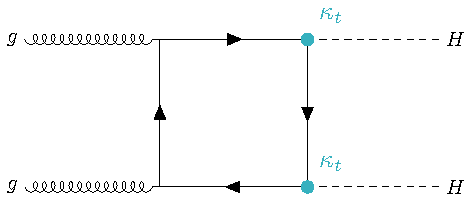
\includegraphics[width=0.45\textwidth]{\figpath/ggF_box.pdf}
        \label{fig:boxFig{\ref{fig:ggF_feyn_dias}}}
    }
    \subfloat[The triangle diagram.]{
        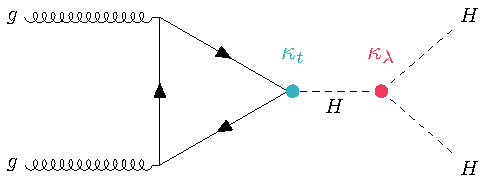
\includegraphics[width=0.45\textwidth]{\figpath/ggF_tri.pdf}
        \label{fig:triangle}
    }
    \caption{The leading order gluon-gluon fusion di-Higgs production Feynman diagrams.}
    \label{fig:ggF_feyn_dias}
\end{figure}

In \Fig{\ref{fig:box_tri}}, you can see the contribution from each of the terms individually, and the interference between the two processes.
In the SM, this process is suppressed to destructive interference between these two diagrams.


\begin{figure}[h]
    \centering
    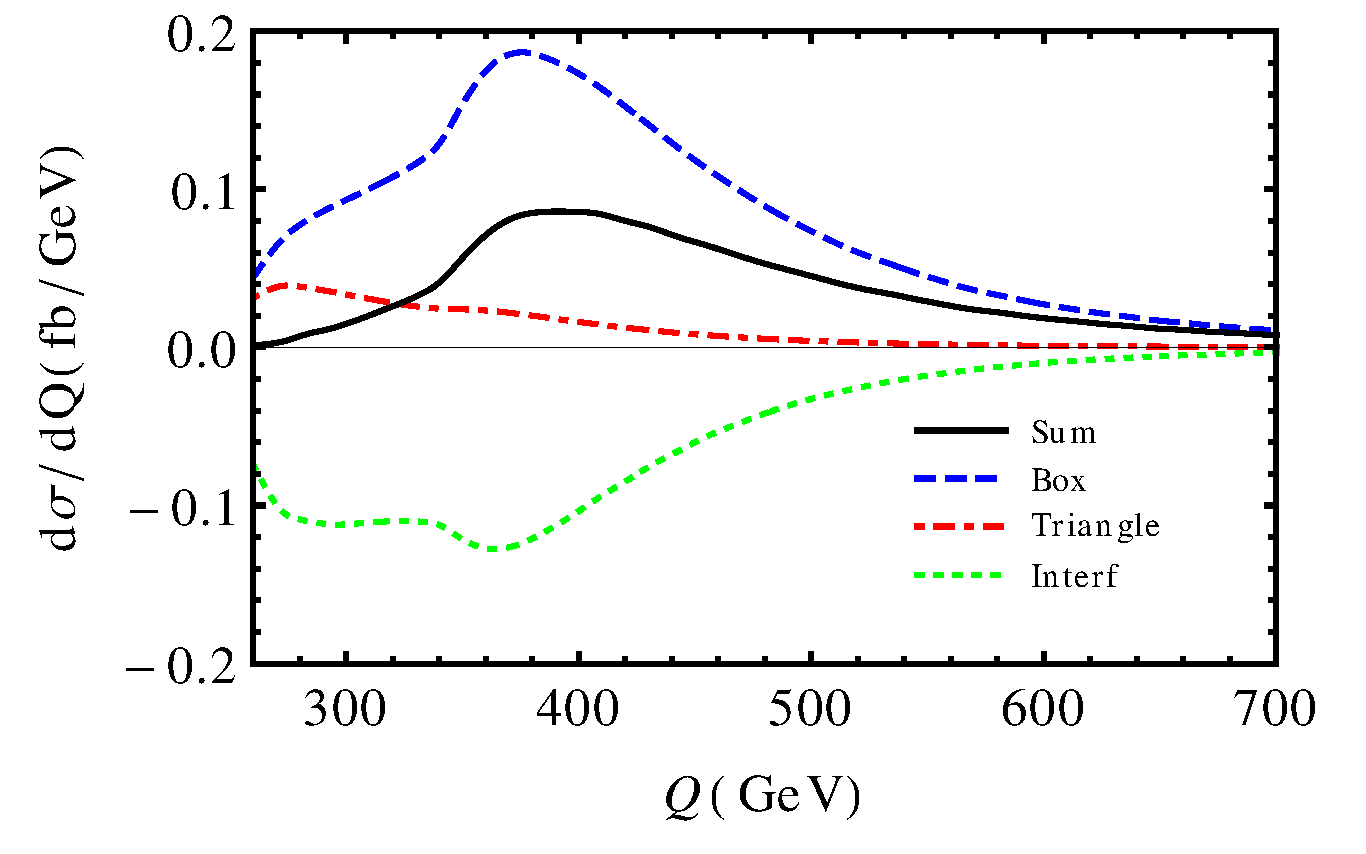
\includegraphics[width=0.8\textwidth]{figures/my_dihiggs/box_triangle_diagram.pdf}
    \caption{Impact of the interference of the box and triangle diagrams for ggF HH production.}
    \label{fig:box-tri}
\end{figure}



%%%%%%%%%%%%%%%%%%%%%%%%
%     VBF
%%%%%%%%%%%%%%%%%%%%%%%%

\textbf{from James - need to rephrase sentences}
The second-leading \HH production process is vector boson fusion (VBF), which has a SM cross-section over an order of magnitude smaller than ggF, at $\sigma_{VBF\,\HH}^{SM} = 1.726$ $\pm 2.1\%$ (PDF+$\alpha_{s}$) $^{+0.03\%}_{-0.04\%}$(Scale)\,fb~\cite{Dreyer_2018} at next-to-next-to-next-to-leading order (N3LO) for a SM Higgs boson with mass of 125 \GeV. 


\begin{figure}[t]
    \centering
    \subfloat[]{
        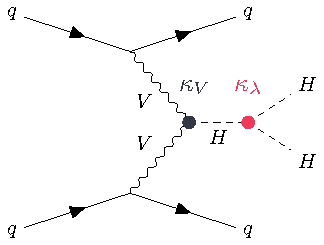
\includegraphics[width=0.33\textwidth]{\figpath/VBF_kvkl.pdf}
        \label{"fig:VBF_kvkl"}
    }
    \subfloat[]{
        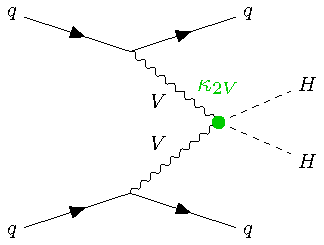
\includegraphics[width=0.33\textwidth]{\figpath/VBF_k2v.pdf}
        \label{"fig:VBF_k2v"}
    }
    \subfloat[]{
        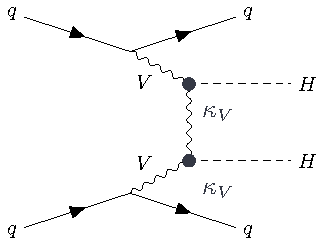
\includegraphics[width=0.33\textwidth]{\figpath/VBF_kvkv.pdf}
        \label{"fig:VBF_kvkv"}
    }
    \caption{The three tree-level vector boson fusion di-Higgs production Feynman diagrams.}
    \label{fig:VBF_feyn_dias}
\end{figure}

\begin{figure}
    \centering
    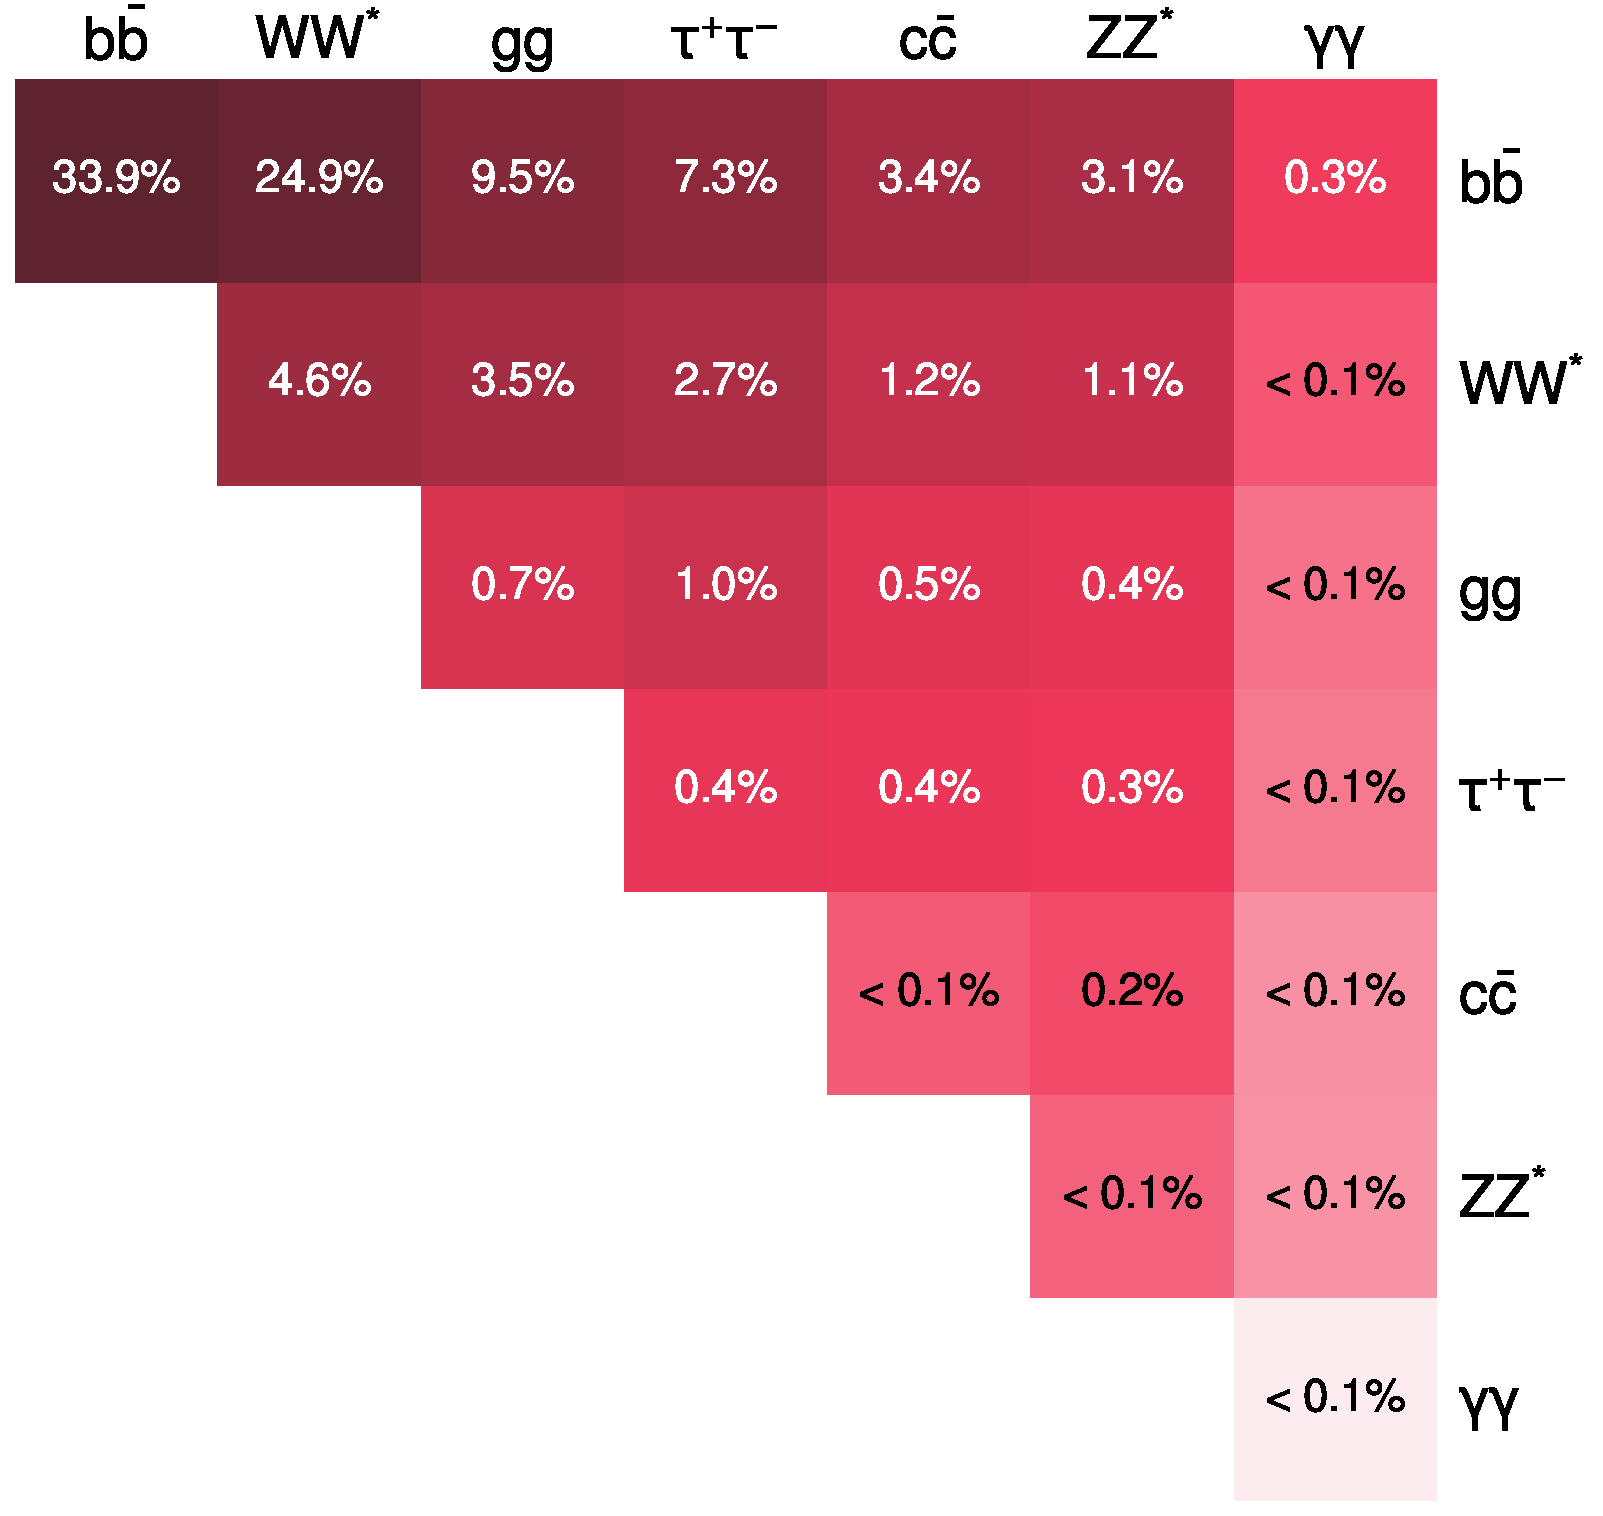
\includegraphics[width=0.7\textwidth]{\figpath/hhbr-dkpink}
    \caption{Branching ratios of the di-Higgs at the LHC.}
    \label{fig:branching-ratios}
\end{figure}

\begin{figure}
    \centering
    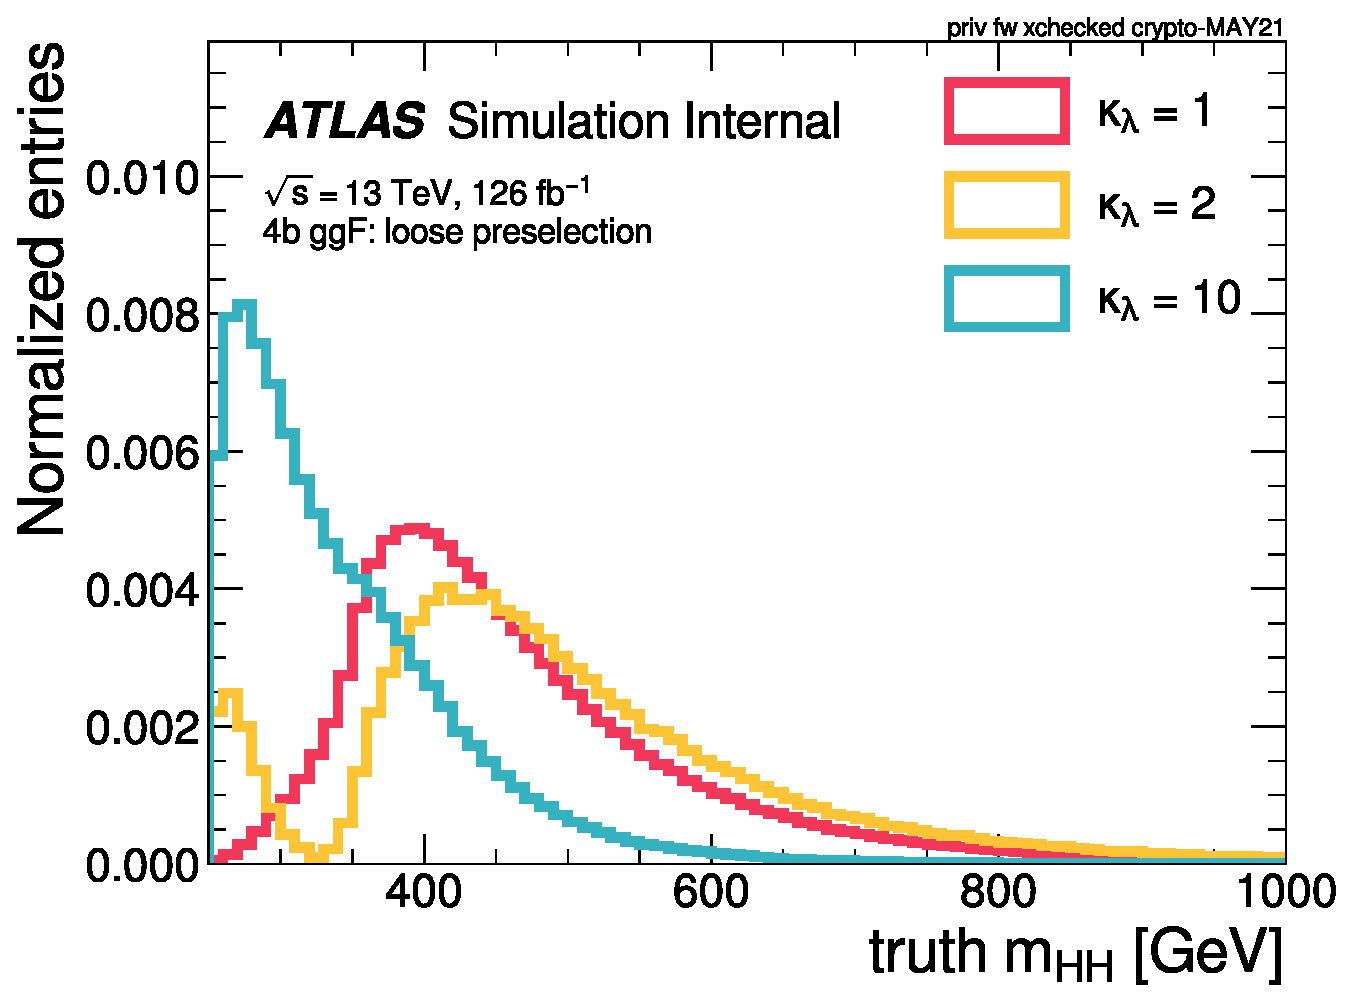
\includegraphics[width=0.7\textwidth]{figures/my_dihiggs/truth_mhh_ggf_common_presel.pdf}
    \caption{Impact of the destructive interference for the \kl variations.}
    \label{fig:truth-hh-presel}
\end{figure}


\section{Datasets and signal parametrization}

\begin{itemize}
	\item Explain why we don't want to generate every single signal
\end{itemize}

\subsection{ggF: histogram based reweighting}

\def\Eq{Eq.~{#1}}

\textbf{Math from my notes reading the 2018 HH comb paper}

Although \Fig{\ref{fig:ggF_feyn_dias}} shows the LO Feynman diagrams, there is a fully differential next-to-leading-order (NLO) calculation, but the terms in this calculation still break down into diagrams in the box and triangle families.
Denoting the sum of the terms in the box and triangle diagrams as $B$ and $T$, respectively.
The impact from a non-SM coupling factors comes as a multiplicative factor for the corresponding vertices, allowing us to write down a combined amplitude (parametrized by $\kappa_t$ and $ \kappa_\lambda$ as:

\begin{equation}
\mathcal{A}(\kappa_t, \kappa_\lambda) &= \kappa_t^2 B + \kappa_t \kappa_\lambda T .
\end{equation}


The ggF cross section is obtained by squaring the amplitude:

\begin{align}
	\sigma(pp \rightarrow HH) \sim |\mathcal{A}^2| = \left( \kappa_t^2 B^* + \kappa_t \kappa_\lambda T^* \right) \left( \kappa_t^2 B + \kappa_t \kappa_\lambda T \right)  \\
	= \kappa_t^4 \left[ |B|^2 + \frac{\kappa_\lambda}{\kappa_t} (B^* T + T^* B) + \left( \frac{\kappa_\lambda}{\kappa_t}  \right)^2 |T|^2 \right] .
	\label{eq:xsec-kl-kt}
\end{align}

The $\kappa_t^4$ term scales the rate of the process. The $2^{nd}$ order $\kappa_\lambda / \kappa_t $ polynomial dictates the way these diagrams interfere, so with 3 different \kl values, we can get any arbitrary \kl value.

To simulate full kinematic sample, consider the basis functions woth $\kappa_t = 1$ and $\kappa_\lambda = 0$ (no triangle diagram), $\kappa_\lambda =1$ and a final (now arbitrary) $\kappa_\lambda = 20$.
 
Plugging these basis points into \Eq{eq:xsec-kl-kt} we get three different differential cross-sections:
 
\begin{align}
|\mathcal{A}(1,0)|^2 &= |B|^2 \\
|\mathcal{A}(1,1)|^2 &= |B|^2 +  (B^* T + T^* B)  + |T|^2  \\
|\mathcal{A}(1,\kappa_0)|^2 &= |B|^2 +  \kappa_0 (B^* T + T^* B)  + \kappa_0^2 |T|^2  \\
\end{align}

\def\a{|\mathcal{A}(1,0)|^2}
\def\b{|\mathcal{A}(1,1)|^2}
\def\c{|\mathcal{A}(1,\kappa_0)|^2}

\def\x{|B|^2} 
\def\y{(B^* T + T^* B) }
\def\z{|T|^2}

Now we solve for $\x$, $\y$, and $\z$ as a function of $\a$, $\b$, and $\c$
Define $x = \x$, $y = \y$, $z=\z$ and $a = \a$, and write this more concisely as a system of linear equations: 

\begin{equation}
\begin{bmatrix} 
a \\ b \\ c
\end{bmatrix}
 = \begin{bmatrix} 
	1 & 0 & 0 \\
	1 & 1 & 1\\
	1 & \kappa_0 & \kappa_0^2 \\
\end{bmatrix}
\begin{bmatrix} 
x \\  y \\ z
\end{bmatrix}
\end{equation}

\begin{equation}
a = x
%
\qquad \text{and} \qquad
%
\begin{bmatrix} 
b - a \\ c-a
\end{bmatrix}
 = \begin{bmatrix} 
	1 & 1\\
	\kappa_0 & \kappa_0^2 \\
\end{bmatrix}
\begin{bmatrix} 
y \\ z
\end{bmatrix}
\end{equation}

Taking the inverse of the matrix to solve for the remaining two terms:

\begin{equation}
\begin{bmatrix} 
y \\ z
\end{bmatrix}
 = \frac{1}{\kappa_0 (\kappa_0 - 1)} \begin{bmatrix} 
	\kappa_0^2  & 1-\\
	-\kappa_0 & 1 \\
\end{bmatrix}
\begin{bmatrix} 
b-a \\ c-a
\end{bmatrix}
\end{equation}


\begin{align}
y &=  \frac{1}{\kappa_0 (\kappa_0 - 1)} \left[  \kappa_0^2 (b-a) - (c-a) \right]  &=  \\
z &=   \frac{1}{\kappa_0 (\kappa_0 - 1)} \left[ - \kappa_0 (b-a) - (c-a)  \right]  &= \\
\end{align}

\textbf{Histogram Reweighting}

We use $\kappa_t = 1$ and $\kappa_\lambda = 0, 1, and 20$.

\textbf{This is an empirical assumption that all of the event level kinematics are \textbf{captured} by the mHH variable!}

\hl{Oh - could I include my plot here instead of MH's?}

\subsection{VBF: event level reweighting}

\section{EFTs}

\section{7.3 Analysis optimization strategy}

\begin{figure}
    \centering
    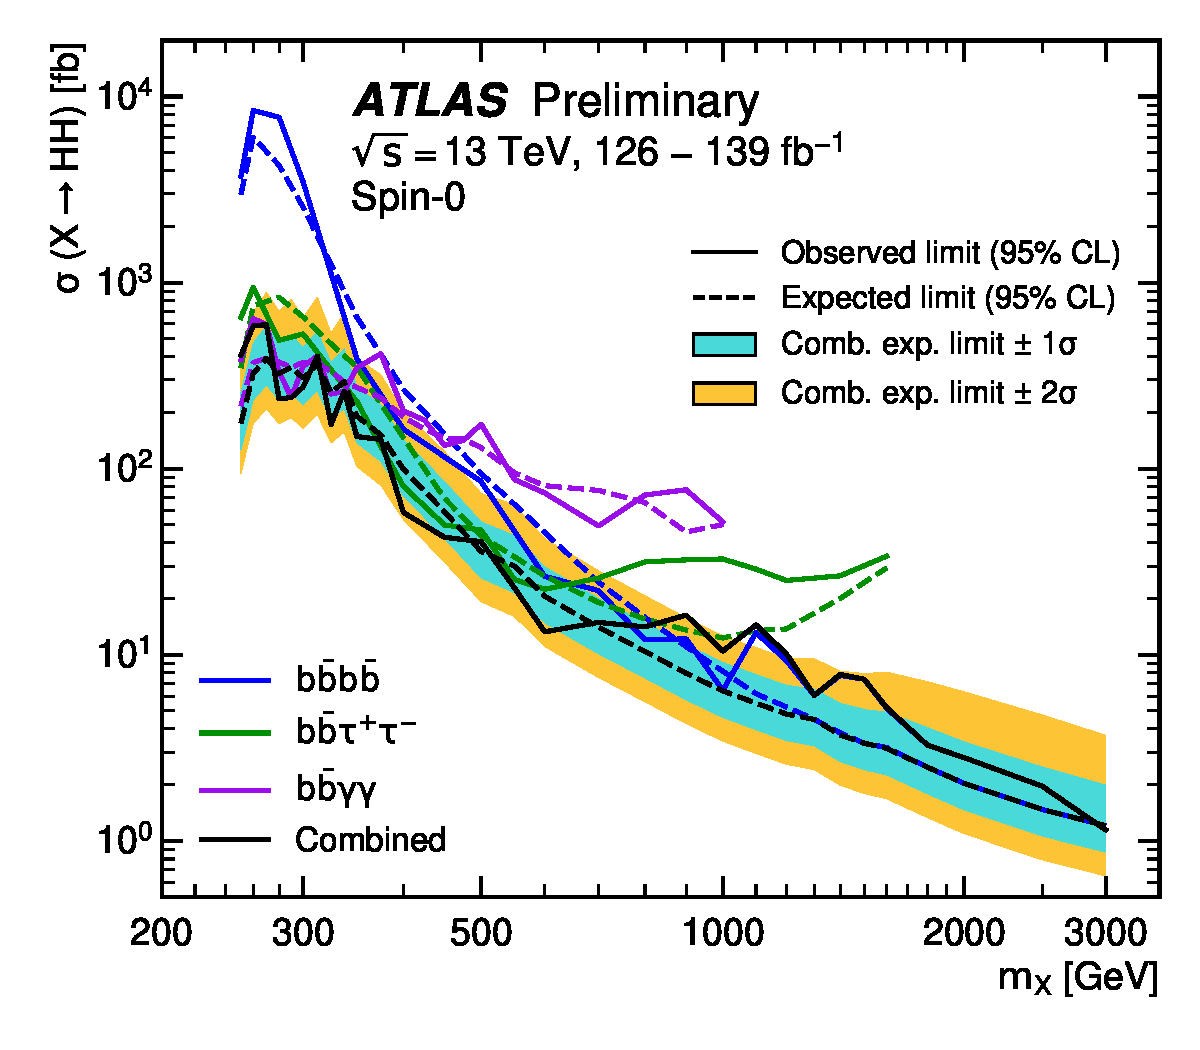
\includegraphics[width=0.9 \textwidth]{figures/ATLAS-CONF-2021-052/fig_08.pdf}
    \caption{Impact of the HH channels in the combination for the resonant scalar mass $m_X$ search \cite{ATLAS-CONF-2021-052} .}
    \label{fig:truth-hh-presel}
\end{figure}


\begin{figure}[h]
    \centering
    \subfloat[SM]{
    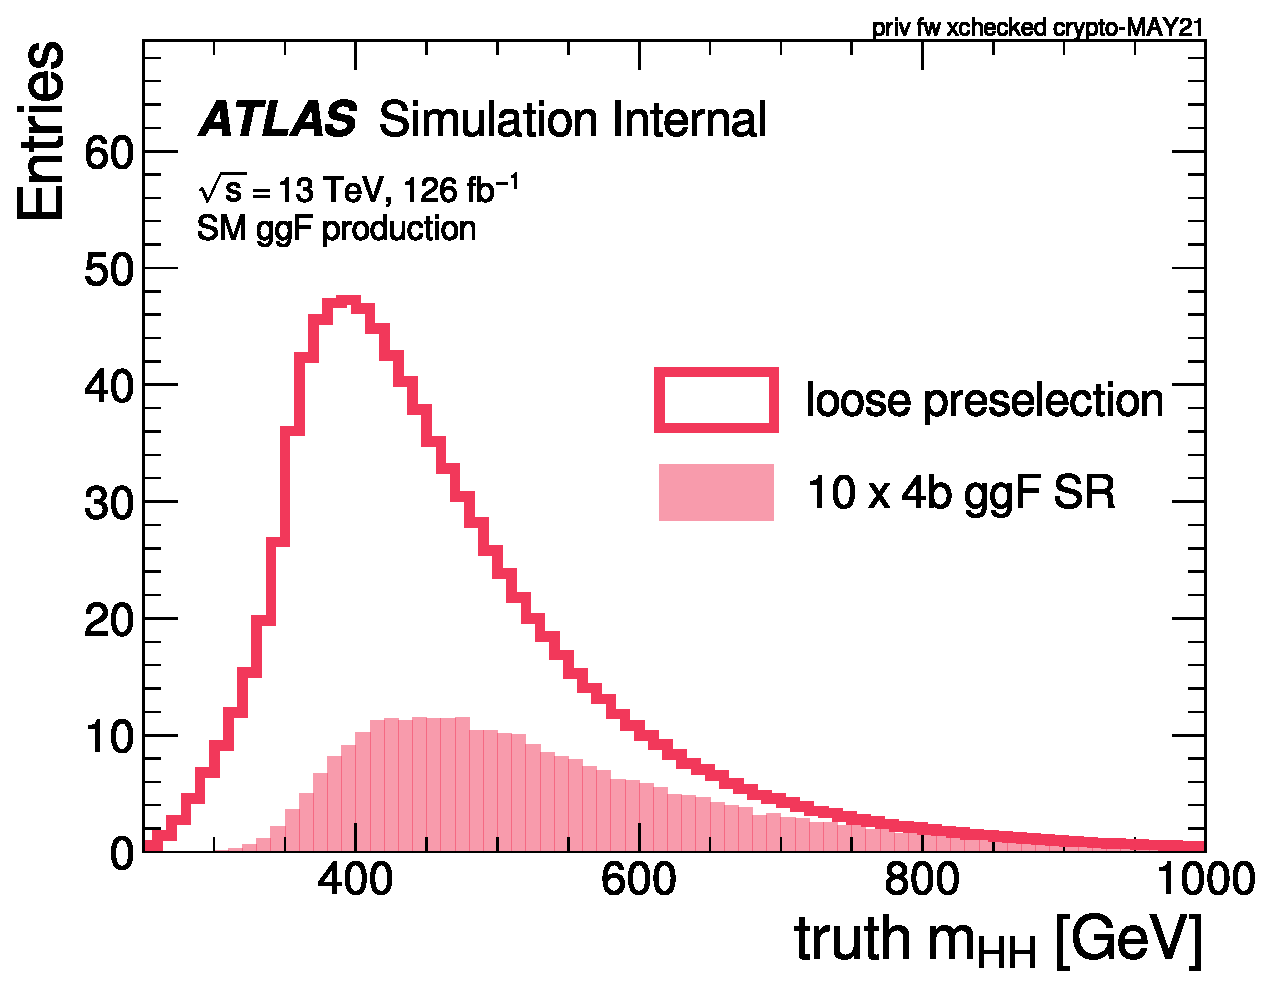
\includegraphics[width=0.33\textwidth]{figures/my_dihiggs/truth_mhh_sm.pdf}
    }
    \subfloat[\kl = 2]{
    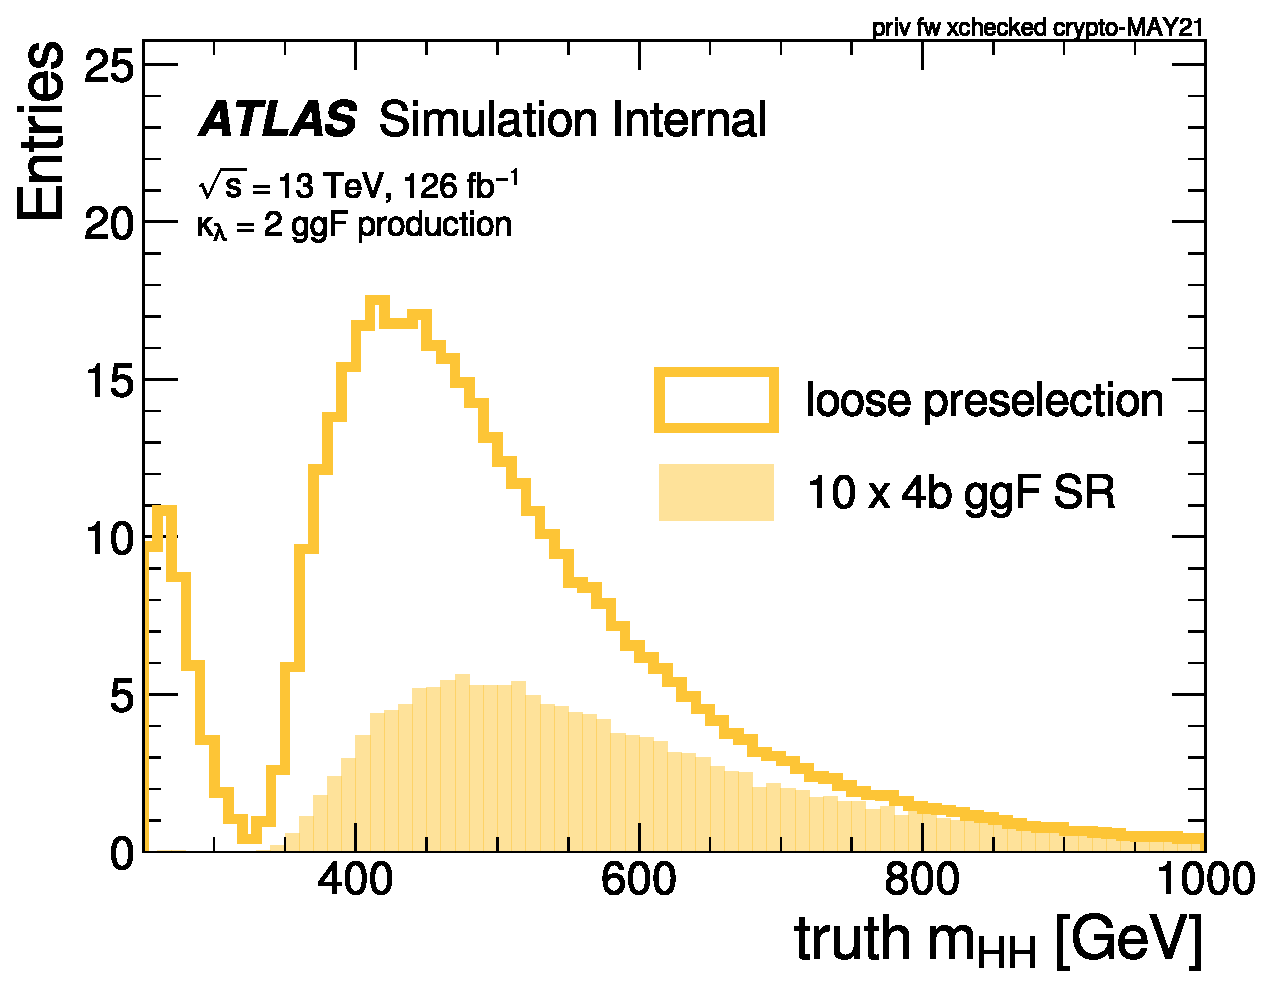
\includegraphics[width=0.33\textwidth]{figures/my_dihiggs/truth_mhh_kl_2.pdf}
    }
    \subfloat[\kl = 10]{
    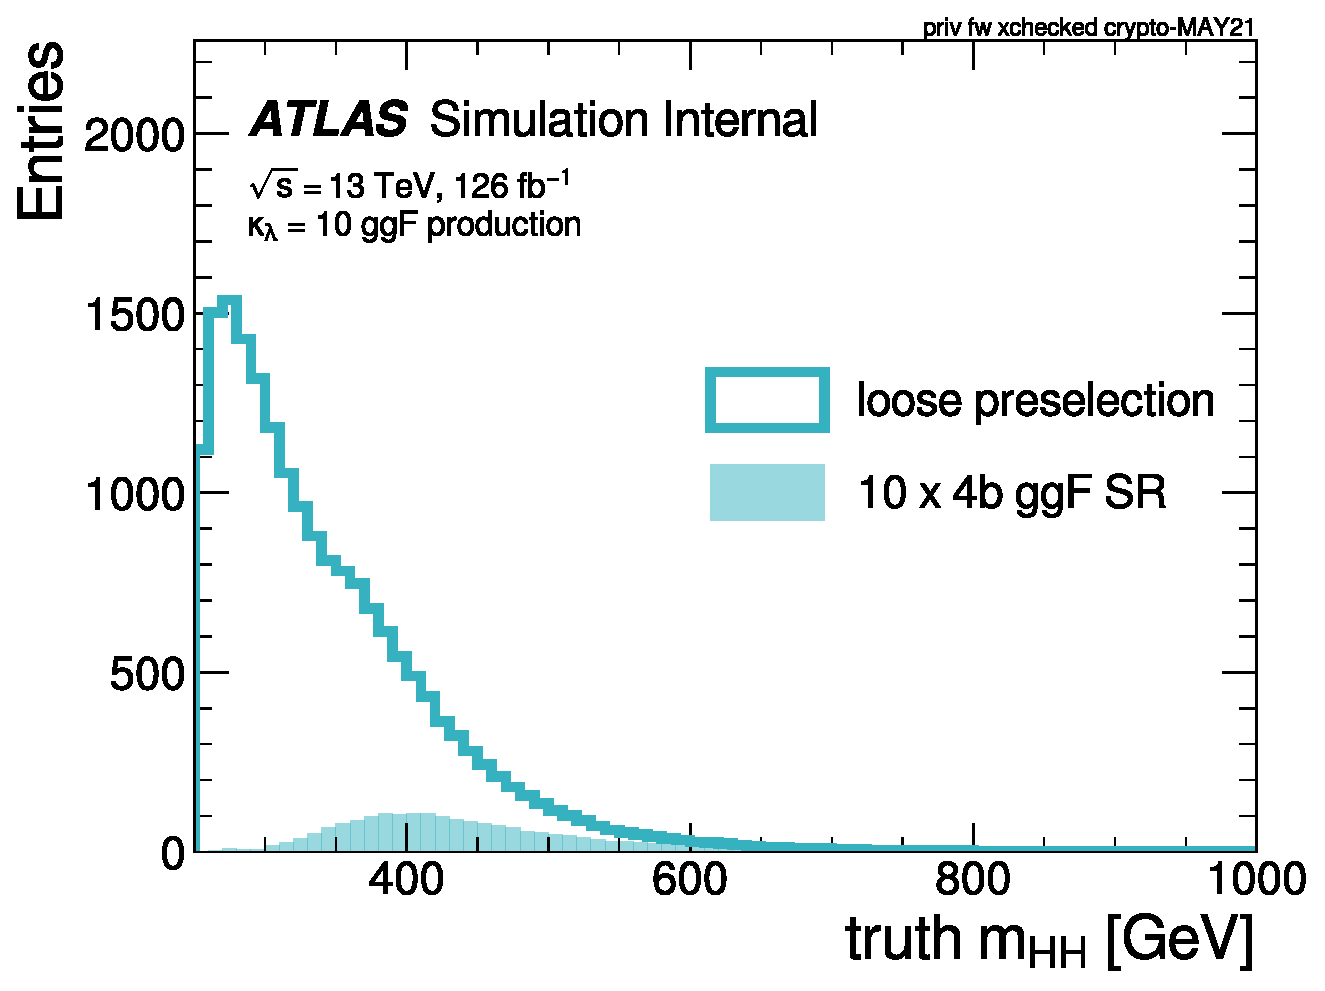
\includegraphics[width=0.33\textwidth]{figures/my_dihiggs/truth_mhh_kl_10.pdf}
    }
    \caption{Impact of the NR analysis selection for selected ggF signals.}
    \label{fig:truth-hh-sel}
\end{figure}


\begin{itemize}
	\item{Show how the sensitivity for 4b is \emph{not as great} at low mass}
\end{itemize}
